\chapter{Partial Derivatives and Gradients}

This chapter will introduce you to partial derivatives and gradients,
equipping you with the tools to study functions of multiple
variables. We will explore how these concepts provide valuable
insights into optimization, vector calculus, and various fields of
science and engineering.

Partial derivatives come into play when dealing with functions that
depend on multiple variables. Unlike ordinary derivatives that
consider changes along a single variable, partial derivatives focus on
how a function changes concerning each individual variable while
holding the others constant. In essence, partial derivatives measure
the rate of change of a function with respect to one variable, while
keeping the other variables fixed.\index{partial derivative}

The notation for a partial derivative of a function $f(x, y, \ldots)$
with respect to a specific variable, say $x$, is denoted as
$\frac{{\partial f}}{{\partial x}}$. Similarly, $\frac{{\partial
    f}}{{\partial y}}$ represents the partial derivative with respect
to $y$, and so on. It is essential to remember that when taking
partial derivatives, we treat the other variables as constants during
the differentiation process.

The gradient is a vector that combines the partial derivatives of a
function. It provides a concise representation of the direction and
magnitude of the steepest ascent or descent of the function. The
gradient vector points in the direction of the greatest rate of
increase of the function. By understanding the gradient, we gain
insights into optimizing functions and finding critical points where
the function reaches maximum or minimum values.\index{gradient}

Throughout this chapter, we will explore the following key topics
related to partial derivatives and gradients:

\begin{itemize}
\item Calculating partial derivatives: We will delve into the
  techniques and rules for computing partial derivatives of various
  functions, including polynomials, exponential functions, and
  trigonometric functions. We will also explore higher-order partial
  derivatives and mixed partial derivatives.

\item Interpreting partial derivatives: Understanding the geometric
  and physical interpretations of partial derivatives is essential. We
  will discuss the notion of tangent planes, directional derivatives,
  and the relationship between partial derivatives and local
  linearity.

\item Gradient vectors and their properties: We will introduce this concept, including it connection to the
  direction of steepest ascent, its relationship with partial
  derivatives, and how it relates to level curves and level surfaces.

\item Applications of partial derivatives and gradients: We will
  explore various applications of these concepts, including
  optimization problems, constrained optimization, tangent planes,
  linear approximations, and their relevance in fields like physics,
  economics, and engineering.
\end{itemize}

By grasping the concepts of partial derivatives and gradients, you
will unlock a powerful mathematical framework for analyzing and
optimizing functions of multiple variables. These tools will equip you
to tackle advanced calculus problems and gain deeper insights into the
behavior of functions in diverse fields.

\section{Calculating Partial Derivatives}
For a function of two variables, $f(x,y)$, we can take the derivative with 
respect to $x$ or with respect to $y$. These are called the \textit{partial 
derivatives} of $f$.\index{partial derivative} Formally, the partial 
derivatives are defined as:

\begin{mdframed}[style = important, frametitle = {Limit Definition of Partial 
Derivatives}]
$$f_x(x, y) = \lim_{h \to 0} \frac{f(x + h, y) - f(x, y)}{h}$$
$$f_y(x, y) = \lim_{h \to 0} \frac{f(x, y + h) - f(x, y)}{h}$$
\end{mdframed}

Let's consider a polynomial function of two variables: $f(x, y) = 3x^2 + y^3 + 
4xy$. We will use the limit definition to find the partial derivative with 
respect to $x$, then compare this to what we already know about derivatives of 
single-variable functions. Recall that if we can describe a function as a sum of 
two other functions, the derivative of the original function is the same as the 
sum of the derivatives of the other functions. That is, 
$$\text{if } f(x) = g(x) + h(x)$$
$$\text{then } f'(x) = g'(x) + h'(x)$$

Let's then define $r(x, y) = 3x^2$, $s(x, y) = y^3$, and $t(x, y) = 4xy$. And 
so $f(x, y) = r(x, y) + s(x, y) + t(x, y)$, which means $f_x(x, y) = r_x(x, y) 
+ s_x(x, y) + t_x(x, y)$. Then,
$$f_x(x, y) = \lim_{h \to 0} \frac{r(x + h, y) - r(x, y)}{h} + \lim_{h \to 0} 
\frac{s(x + h, y) - s(x, y)}{h} + \lim_{h \to 0} \frac{t(x + h, y) - t(x, y)}{
h}$$
$$= \lim_{h \to 0} \frac{3(x + h)^2 - 3x^2}{h} + \lim_{h \to 0} \frac{y^3 - 
y^3}{h} + \lim_{h \to 0} \frac{4(x + h)y - 4xy}{h}$$
$$= \lim_{h \to 0} \frac{3x^2 + 6xh + h^2 - 3x^2}{h} + 0 + \lim_{h \to 0} 
\frac{4xy + 4hy - 4xy}{h}$$

Notice that $s_x(x, y) = 0$. This term only had $y$, and its derivative with 
respect to $x$ is zero. Continuing, 

$$f_x(x, y) = \lim_{h \to 0} \frac{6xh + h^2}{h} + \lim_{h \to 0} \frac{4hy}{h}
= \lim_{h \to 0} 6x + h + \lim_{h \to 0} 4y$$
$$= 6x + 4y$$

As you can see, $r_x(x, y) = 6x$ and $t_x(x, y) = 4y$. Recall the polynomial 
rule for single derivatives. The derivative of $3x^2$ is $6x$, which is also 
what we see with the partial derivative in this case. What about the other 
term, $4xy$? Well, we know the derivative of $bx$, where $b$ is a constant, is 
$b$. The partial derivative of $4xy$ with respect to $x$ being $4y$ suggests 
the rule for determining partial derivatives:

\begin{mdframed}[style = important, frametitle = {Rule for Finding Partial 
Derivatives of $f(x, y)$}]
\begin{enumerate}
    \item To find the partial derivative with respect to $x$, $f_x$, treat $y$ 
    as a constant and differentiate with respect to $x$.
    \item To find the partial derivative with respect to $y$, $f_y$, treat $x$ 
    as a constant and differentiate with respect to $y$.
\end{enumerate}
\end{mdframed}

Let's check this by predicting $f_y$, then using the limit definition to 
confirm our prediction. Applying the polynomial rule, we predict that $f_y$ is:
$$f_y(x, y) = 3y^2 + 4x$$

Which we found by treating $x$ as a constant and taking the derivative of each 
term with respect to $y$. Let's see if we get the same result using the limit 
definition of the derivative with respect to $y$:
$$f_y(x, y) = \lim_{h \to 0} \frac{f(x, y + h) - f(x, y)}{h}$$
$$= \lim_{h \to 0} \frac{\left[3x^2 + \left(y + h \right)^3 + 4x \left(y + h 
\right) \right] - \left[ 3x^2 + y^3 + 4xy \right]}{h}$$
$$= \lim_{h \to 0} \frac{3x^2 + y^3 + 3y^2h + 3yh^2 + h^3 + 4xy + 4xh - 3x^2 - 
y^3 - 4xy}{h}$$
$$= \lim_{h \to 0} \frac{3y^2h + 3yh^2 + h^3 + 4xh}{h} = \lim_{h \to 0} 3y^2 + 
3yh + h^2 + 4x = 3y^2 + 4x$$

Which is our expected result. In summary, you find the partial derivative with 
respect to a particular variable by treating all the other variables as 
constants and differentiating with respect to the particular variable, applying
the rules of differentiation you've already learned. 

\subsection{Partial Derivative Notation}
There are many ways to denote a partial derivative. We've already seen one way,
$f_x$ and $f_y$. Another common notation uses a lowercase Greek letter delta, 
and a further uses capital D. They are shown below:

\begin{mdframed}[style = important, frametitle = {Partial Derivative Notations}]
$$f_x(x, y) = f_x = \frac{\partial f}{\partial x} = \frac{\partial}{\partial x}
f(x, y) = D_x f$$
$$f_y(x, y) = f_y = \frac{\partial f}{\partial y} = \frac{\partial}{\partial y}
f(x, y) = D_y f$$
\end{mdframed}

\begin{Exercise}[title = {First Partial Derivatives}, label = first]
Find $f_x$ and $f_y$ for the following functions.
\begin{enumerate}
\item $f(x, y) = 3x^4 + 4x^2y^3$
\item $f(x, y) = xe^{-y}$
\item $f(x, y) = \sqrt{3x + 4y^2}$
\item $f(x, y) = \sin{x^2y}$
\item $f(x, y) = \ln{ \left(x^y \right)}$
\end{enumerate}
\vspace{50mm}
\end{Exercise}

\begin{Answer}[ref = first]
\begin{enumerate}
    \item $f_x(x, y) = \frac{\partial}{\partial x} \left[ 3x^4 + 4x^2y^3 
    \right] = 12x^3 + 8y^3$ and $f_y(x, y) = \frac{\partial}{\partial y} 
    \left[ 3x^4 + 4x^2y^3 \right] = 12x^2y^2$
    \item $f_x(x, y) = \frac{\partial}{\partial x} \left(xe^{-y} \right) = 
    e^{-y}$ and $f_y(x, y) = \frac{\partial}{\partial y} \left(xe^{-y} \right) 
    = -xe^{-y}$
    \item $f_x(x, y) = \frac{\partial}{\partial x} \sqrt{3x + 4y^2} = \left( 
    \frac{1}{2\sqrt{3x + 4y^2}} \right) \left( \frac{\partial}{\partial x } 
    \left(3x + 4y^2 \right) \right) = \frac{3}{2\sqrt{3x + 4y^2}}$ and $f)y(x, 
    y) = \frac{\partial}{\partial y} \sqrt{3x + 4y^2} = \frac{1}{2\sqrt{3x + 
    4y^2}} \left( \frac{\partial}{\partial y} \left(3x + 4y^2 \right) \right) 
    = \frac{8y}{2\sqrt{3x + 4y^2}} = \frac{4y}{\sqrt{3x + 4y^2}}$
    \item $f_x(x, y) = \frac{\partial}{\partial x} \sin{ \left(x^2y \right)} = 
    \cos{\left( x^2y \right)} \left( \frac{\partial}{\partial x} \left(x^2y 
    \right) \right) = 2xy\cos{\left(x^2y \right)}$ and $f_y(x, y) = \frac{
    \partial}{\partial y} \sin{ \left(x^2y \right)} = \cos{ \left(x^2y \right)}
    \left( \frac{\partial}{\partial y} \left(x^2 y \right) \right) = x^2\cos{ 
    \left( x^2 y \right)}$
    \item $f_x(x, y) = \frac{\partial}{\partial x} \ln{ \left( x^y \right)} = 
    \frac{\partial}{\partial x} \left(y \ln{x} \right) = \frac{y}{x}$ and $f_y(
    x, y) = \frac{\partial}{\partial y} \left(y \ln{x} \right) = \ln{x}$
\end{enumerate}
\end{Answer}

\subsection{Partial Derivatives of Functions of More than Two Variables}
The above method of determining partial derivatives applies to functions with 
three, four, or any number of variables.

\textbf{Example}: Find all the first derivatives of the function $f(x, y, z) = 
y\cos{ \left(x^2 + 3z \right)}$. 

\textbf{Solution}: 
$$\frac{\partial f}{\partial x} = \frac{\partial}{\partial x} \left[ y \cos{ 
\left(x^2 + 3z \right)} \right] = -y\sin{\left(x^2 + 3z \right)} \left( \frac{
\partial}{\partial x} \left( x^2 + 3z \right) \right)$$
$$\frac{\partial f}{\partial x} = -2xy \sin{ \left( x^2 + 3z \right)}$$

And
$$\frac{\partial f}{\partial y} = \frac{\partial}{\partial y} \left[ y\cos{ 
\left(x^2 + 3z \right)} \right]$$
$$\frac{\partial f}{\partial y} = \cos{ \left(x^2 + 3z \right)}$$

And
$$\frac{\partial f}{\partial z} = \frac{\partial}{\partial z} \left[ y \cos{ 
\left(x^2 + 3z \right)} \right] = -y\sin{ \left(x^2 + 3z \right)} \left( \frac{
\partial}{\partial z} \left( x^2 + 3z \right) \right)$$
$$\frac{\partial f}{\partial z} = -3y \sin{ \left(x^2 + 3z \right)}$$

\begin{Exercise}[title = {Partial Derivatives with 3 or More Variables}, 
label = three]
Find all first partial derivatives of the following functions.
\begin{enumerate}
\item $f = \sin{\left( x^2 - y^2 \right)} \cos{\left( \sqrt{z} \right)}$
\item $q = \sqrt[3]{t^3 + u^3\sin{\left(5v \right)}}$
\item $w = x^z y^x$
\end{enumerate}
\vspace{100mm}
\end{Exercise}

\begin{Answer}[ref = three]
\begin{enumerate}
    \item Finding $f_x$:
    $$f_x = \frac{\partial}{\partial x} \left[ \sin{ \left( x^2 - y^2 \right)} 
    \cos{ \left( \sqrt{z} \right)} \right] = \cos{ \left(x^2 - y^2 \right)} 
    \cos{ \left( \sqrt{z} \right)} \left[ \frac{\partial}{\partial x} \left( 
    x^2 - y^2 \right) \right]$$
    $$f_x = 2x \cos{ \left(x^2 - y^2 \right)} \cos{ \left( \sqrt{z} \right) }$$

    Finding $f_y$:
    $$f_y = \frac{\partial}{\partial y} \left[ \sin{\left( x^2 - y^2 \right)} 
    \cos{\left( \sqrt{z} \right)} \right] = \cos{ \left( x^2 - y^2 \right)} 
    \cos{ \left( \sqrt{z} \right) } \left[ \frac{\partial}{\partial y} \left(
    x^2 - y^2 \right) \right]$$
    $$f_y = -2y \cos{ \left( x^2 - y^2 \right)} \cos{\left( \sqrt{z} \right)}$$

    Finding $f_z$:
    $$f_z = \frac{\partial}{\partial z} \left[ \sin{\left( x^2 - y^2 \right)} 
    \cos{\left( \sqrt{z} \right)} \right] = \sin{ \left( x^2 - y^2 \right) } 
    \left( -\sin{ \sqrt{z} } \right) \cdot \left( \frac{\partial}{\partial z} 
    \sqrt{z} \right)$$
    $$f_z = \frac{-\sin{ \left( x^2 - y^2 \right)} \sin{ \left( \sqrt{z} 
    \right)}}{2\sqrt{z}}$$

    \item Finding $q_t$:
    $$q_t = \frac{\partial}{\partial t} \sqrt[3]{t^3 + u^3 \sin{ \left(5v 
    \right)}} = \frac{1}{3 \left(t^3 + u^3 \sin{ \left( 5v \right)} \right)^{
    2/3}} \left( \frac{\partial}{\partial t} \left(t^3 + u^3 \sin{ \left(5v 
    \right)} \right) \right)$$
    $$q_t = \frac{t^2}{\left( t^3 + u^3 \sin{\left(5v \right)} \right)^{2/3}}$$

    Finding $q_u$:
    $$q_u = \frac{\partial}{\partial u} \sqrt[3]{t^3 + u^3\sin{\left(5v \right)
    }} = \frac{1}{3 \left( t^3 + u^3 \sin{ \left(5v \right)} \right)^{2/3}} 
    \left( \frac{\partial}{\partial u} \left(t^3 + u^3 \sin{ \left(5 v \right)}
    \right) \right) $$
    $$q_u = \frac{u^2 \sin{ \left( 5v \right) }}{\left( t^3 + u^3 \sin{ \left( 
    5v \right)} \right)^{2/3}}$$

    Finding $q_v$:
    $$q_v = \frac{\partial}{\partial v} \sqrt[3]{t^3 + u^3\sin{\left(5v \right)
    }} = \frac{1}{3 \left(t^3 + u^3 \sin{\left( 5v \right)} \right)^{2/3}} 
    \left( \frac{\partial}{\partial v} \left(t^3 + u^3 \sin{ \left( 5v \right)}
    \right) \right)$$
    $$q_v = \frac{u^3 \cos{ \left( 5v \right)}}{3 \left( t^3 + u^3 \sin{ \left(
    5v \right)} \right)^{2/3}} \left( \frac{\partial}{\partial v} \left( 5v 
    \right) \right) = \frac{5u^3 \cos{ \left( 5v \right)}}{3 \left( t^3 + u^3 
    \sin{ \left( 5v \right)} \right)^{2/3}}$$

    \item Finding $w_x$:
    $$w_x = \frac{\partial}{\partial x} \left( x^z y^x \right) = \left( x^z 
    \right) \cdot \left( \frac{\partial}{\partial x} y^x \right) + \left( y^x 
    \right) \cdot \left( \frac{\partial}{\partial x} x^z \right)$$
    $$w_x = \left(x^z \right) \left( \ln{ \left( y \right)} y^x \right) + 
    \left( y^x \right) \left(zx^{z-1} \right) = \left(x^{z-1} y^x \right) 
    \left( x\ln{\left( y \right)} + z \right)$$

    Finding $w_y$:
    $$w_y = \frac{\partial}{\partial y} \left(x^z y^x \right) = \left( x^z 
    \right) \left( \frac{\partial}{\partial y} y^x \right) = x^z \left( xy^{
    x - 1} \right)$$
    $$w_y = x^{z + 1} y^{x - 1}$$

    Finding $w_z$:
    $$w_z = \frac{\partial}{\partial z} \left( x^z y^x \right) = \left( y^x 
    \right) \left( \frac{\partial}{\partial z} x^z \right) = \left( y^x \right)
    \left( \ln{\left(x \right)} x^z \right)$$
    $$w_z = \ln{ \left(x \right)} y^x x^z$$
\end{enumerate}
\end{Answer}

\subsection{Higher Order Partial Derivatives}
Just like with single-variable equations, we can take the partial derivative 
more than once. There are also several notations for second partial derivatives.

\begin{mdframed}[style = important, frametitle = 
{Second Partial Derivative Notation}]
$$(f_x)_x = f_{xx} = \frac{\partial}{\partial x} \left( \frac{\partial f}{
\partial x} \right) = \frac{\partial^2 f}{\partial x^2}$$
$$(f_x)_y = f_{xy} = \frac{\partial}{\partial y} \left( \frac{\partial f}{
\partial x} \right) = \frac{\partial^2 f}{\partial y \partial x}$$
$$(f_y)_x = f_{yx} = \frac{\partial}{\partial x} \left( \frac{\partial f}{
\partial y} \right) = \frac{\partial^2 f}{\partial x \partial y}$$
$$(f_y)_y = f_{yy} = \frac{\partial}{\partial y} \left( \frac{\partial f}{
\partial y} \right) = \frac{\partial^2 f}{\partial y^2}$$
\end{mdframed}

Notice that for $\left( \partial^2 f / \partial y \partial x \right)$, we 
first take the derivative with respect to $x$, then with respect to $y$. 

\textbf{Example}: Find all the second order partial derivatives of $f(x, y) = 
2x^2 - x^3y^2 + y^3$.

\textbf{Solution}: We begin by finding $f_x$ and $f_y$:
$$f_x(x, y) = 4x - 3x^2y^2$$
$$f_y(x, y) = -2x^3y + 3y^2$$

We then take another partial derivative to find all the second order partial 
derivatives:
$$f_{xx}(x, y) = \frac{\partial}{\partial x}f_x(x, y) = \frac{\partial}{
\partial x} \left( 4x - 3x^2y^2 \right) = 4 - 6xy^2$$
$$f_{xy}(x, y) = \frac{\partial}{\partial y}f_x(x, y) = \frac{\partial}{
\partial y} \left( 4x - 3x^2y^2 \right) = -6x^2y$$
$$f_{yx}(x, y) = \frac{\partial}{\partial x}f_y(x, y) = \frac{\partial}{
\partial x} \left( -2x^3y + 3y^2 \right) = -6x^2y$$
$$f_{yy}(x, y) = \frac{\partial}{\partial y}f_y(x, y) = \frac{\partial}{
\partial y} \left( -2x^3y + 3y^2 \right) = -2x^3 + 6y$$

What do you notice about $f_{xy}$ and $f_{yx}$? They are the same! This is not 
a coincidence of the particular function used in the example. For most 
functions, $f_{xy} = f_{yx}$, as stated by Clairaut's theorem\index{Clairaut's 
theorem}.

\begin{mdframed}[style = important, frametitle = {Clairaut's Theorem}]
If $f$ is defined on a disk $D$ and $f_{xy}$ and $f_{yx}$ are both continuous 
on $D$, then $f_{xy} = f_{yx}$ on $D$.
\end{mdframed}

This is also true for third, fourth, and higher-order derivatives. 

\begin{Exercise}[title = {Clairaut's Theorem}, label = clairaut]
Show that Clairaut's theorem holds for the following functions (show that 
$f_{xy} = f_{yx}$). 
\begin{enumerate}
    \item $f(x, y) = e^{2xy} \sin{x}$
    \item $f(x, y) = \frac{x^2}{x + y}$
    \item $f(x, y) = \ln{\left( 2x + 3y \right)}$
\end{enumerate}
\vspace{70mm}
\end{Exercise}

\begin{Answer}
\begin{enumerate}
    \item $f_{xy} = \frac{\partial}{\partial y} \left( 
    \frac{\partial}{\partial x} f(x, y) \right) = \frac{\partial}{\partial y} 
    \left[ \frac{\partial}{\partial x} \left( e^{2xy} \sin{x} \right) \right] 
    = \frac{\partial}{\partial y} \left[ \left(e^{2xy} \right) \left( 
    \frac{\partial}{\partial x}\sin{x} \right) + \left( \sin{x} \right) \left( 
    \frac{\partial}{\partial x} e^{2xy} \right) \right] = 
    \frac{\partial}{\partial y} \left[ e^{2xy}\cos{x} + 2ye^{2xy}\sin{x} 
    \right] = \frac{\partial}{\partial y} \left( e^{2xy} \cos{x} \right) + 
    \frac{\partial}{\partial y} \left( 2ye^{2xy} \sin{x} \right) = 2xe^{2xy}
    \cos{x} + \left( 2y \right) \left( \frac{\partial}{\partial y}e^{2xy}
    \sin{x} \right) + \left(e^{2xy} \sin{x} \right) \left( 
    \frac{\partial}{\partial y} 2y \right) = 2xe^{2xy}\cos{x} + 4xye^{2xy}
    \sin{x} + 2e^{2xy}\sin{x}$

    $f_{yx} = \frac{\partial}{\partial x} \left( \frac{\partial}{\partial y} 
    f(x, y) \right) = \frac{\partial}{\partial x} \left[ \frac{\partial}{
    \partial y} \left(e^{2xy} \sin{x} \right) \right] = \frac{\partial}{
    \partial x} \left( 2xe^{2xy} \sin{x} \right) = \left(2x \right) \left[ 
    \frac{\partial}{\partial x} \left( e^{2xy} \sin{x} \right) \right] + \left(
    e^{2xy} \sin{x} \right) \left( \frac{\partial}{\partial x} 2x \right) = 
    \left(2x \right) \left[ \left( e^{2xy} \right) \left( \frac{\partial}{
    \partial x} \sin{x} \right) + \left( \sin{x} \right) \left( \frac{
    \partial}{\partial x}e^{2xy} \right) \right] + 2e^{2xy}\sin{x} = 2xe^{2xy}
    \cos{x} + 4xye^{2xy}\sin{x} + 2e^{2xy}\sin{x} = f_{xy}$

    \item $f_{xy} = \frac{\partial}{\partial y} \left( \frac{\partial}{
    \partial x}f(x, y) \right) = \frac{\partial}{\partial y} \left[ \frac{
    \partial}{\partial x} \left( \frac{x^2}{x + y} \right) \right] = \frac{
    \partial}{\partial y} \left[ \frac{(x + y) \left( 2x \right) - x^2 \left(
    1 \right)}{\left( x + y \right)^2} \right] = \frac{\partial}{\partial y} 
    \left[ \frac{x^2 + 2xy}{\left( x + y \right)^2} \right] = \frac{\left( x + 
    y \right)^2 \left( 2x \right) - \left( x^2 + 2xy \right) \left(2(x + y) 
    \right)}{\left( x + y \right)^4} = \frac{\left( x^2 + 2xy + y^2 \right) 
    \left( 2x \right) - \left( x^2 + 2xy \right) \left( 2x + 2y \right)}{\left(
    x + y \right)^4} = \frac{2x^3 + 4x^2y + 2xy^2 - 2x^3 - 2x^2y - 4x^2y - 
    4xy^2}{\left( x + y \right)^4} = \frac{-2x^2y - 2xy^2}{\left( x + y \right)
    ^4}$

    $f_{yx} = \frac{\partial}{\partial x} \left( \frac{\partial}{\partial y} 
    f(x, y) \right) = \frac{\partial}{\partial x} \left[ \frac{\partial}{
    \partial y} \left( \frac{x^2}{x + y} \right) \right] = \frac{\partial}{
    \partial x} \left[ \frac{-x^2}{\left( x + y \right)^2} \right] = \frac{
    \left(x + y \right)^2 \left( -2x \right) - \left( -x^2 \right) \left( 2 
    (x + y ) \right)}{\left( x + y \right)^4} = \frac{\left(x^2 + 2xy + y^2 
    \right) \left(-2x \right) + x^2 \left(2x + 2y \right)}{\left( x + y \right)
    ^4} = \frac{-2x^3 - 4x^2y - 2xy^2 + 2x^3 + 2x^2y}{\left( x + y \right)^4} =
    \frac{-2x^2y - 2xy^2}{\left( x + y \right)^4} = f_{xy}$

    \item $f_{xy} = \frac{\partial}{\partial y} \left( \frac{\partial}{
    \partial x}f(x, y) \right) = \frac{\partial}{\partial y} \left[ \frac{
    \partial}{\partial x} \left( \ln{\left(2x + 3y \right)} \right) \right] = 
    \frac{\partial}{\partial y} \left[ \frac{2}{2x + 3y} \right] = \frac{-2 
    \left( 3 \right)}{ \left( 2x + 3y \right)^2} = \frac{-6}{\left( 2x + 3y 
    \right)^2}$

    $f_{yx} = \frac{\partial}{\partial x} \left( \frac{\partial}{\partial y}
    f(x, y) \right) = \frac{\partial}{\partial x} \left[ \frac{\partial}{
    \partial y} \left( \ln{ \left( 2x + 3y \right)} \right) \right] = \frac{
    \partial}{\partial x} \left( \frac{3}{2x + 3y} \right) = \frac{-3(2)}{
    \left( 2x + 3y \right)^2} = \frac{-6}{\left( 2x + 3y \right)} = f_{xy}$
\end{enumerate}
\end{Answer}

\begin{Exercise}[title = {Second Order Partial Derivatives}, label = second]
Find all second order partial derivatives of the function. 
\begin{enumerate}
\item $f(x, y) = x^5y^2 - 3x^3y^2$
\item $v = \sin{\left( p^3 + q^2 \right)}$
\item $T = e^{-3r} \cos{\theta^2}$
\end{enumerate}
\vspace{75mm}
\end{Exercise}

\begin{Answer}[ref = second]
\begin{enumerate}
\item $f_{xx} = \frac{\partial}{\partial x} \left( \frac{\partial}{\partial x}
f(x, y) \right) = \frac{\partial}{\partial x} \left[ \frac{\partial}{\partial 
x} \left( x^5y^2 - 3x^3y^2 \right) \right] = \frac{\partial}{\partial x} \left(
5x^4y^2 - 9x^2y^2 \right) = 20x^3y^2 - 18xy^2$. 

$f_{xy} = f_{yx} = \frac{\partial}{\partial y} \left( \frac{\partial}{\partial 
x}f(x, y) \right) = \frac{\partial}{\partial y} \left[ \frac{\partial}{\partial
x} \left( x^5y^2 - 3x^3y^2 \right) \right] = \frac{\partial}{\partial y} \left(
5x^4y^2 - 9x^2y^2 \right) = 10x^4y - 18x^2y$. 

$f_{yy} = \frac{\partial}{\partial y} \left( \frac{\partial}{\partial y} 
f(x, y) \right) = \frac{\partial}{\partial y} \left[ \frac{\partial}{\partial 
y} \left( x^5y^2 - 3x^3y^2 \right) \right] = \frac{\partial}{\partial y} \left(
2x^5y - 6x^3y \right) = 2x^5 - 6x^3$. 

\item $v_{pp} = \frac{\partial}{\partial p} \left( \frac{\partial}{\partial p}
v(p, q) \right) = \frac{\partial}{\partial p} \left[ \frac{\partial}{\partial 
p} \left( \sin{ \left(p^3 + q^2 \right)} \right) \right] = \frac{\partial}{
\partial p} \left( \cos{ \left( p^3 + q^2 \right)} \left( 3p^2 \right) \right) 
= \cos{ \left(p^3 + q^2 \right)} \cdot \frac{\partial}{\partial p} \left( 3p^2 
\right) + 3p^2 \cdot \frac{\partial}{\partial p} \left(\cos{ \left(p^3 + q^2 
\right)} \right)$

$v_{pq} = v_{qp} = \frac{\partial}{\partial q} \left( \frac{\partial}{\partial 
p} v(p, q) \right) = \frac{\partial}{\partial q} \left[ \frac{\partial}{
\partial p} \left( \sin{ \left(p^3 + q^2 \right)} \right) \right] = \frac{
\partial}{\partial q} \left( \cos{ \left( p^3 + q^2 \right)} \left( 3p^2 
\right) \right) = \cos{ \left( p^3 + q^2 \right)} \frac{\partial}{\partial q} 
\left( 3p^2 \right) + 3p^2 \frac{\partial}{\partial q} \cos{ \left( p^3 + q^2 
\right)} = 0 + 3p^2 \left(-\sin{ \left( p^3 + q^2 \right)} \right) \left( 
\frac{\partial}{\partial q} \left(p^3 + q^2 \right) \right) = -6 p^2 q \sin{ 
\left(p^3 + q^2 \right)}$

$v_{qq} = \frac{\partial}{\partial q} \left( \frac{\partial}{\partial q}v(p, q)
\right) = \frac{\partial}{\partial q} \left[ \frac{\partial}{\partial q} \left(
\sin{\left( p^3 + q^2 \right)} \right) \right] = \frac{\partial}{\partial q} 
\left[ 2q\cos{ \left(p^3 + q^2 \right)} \right] = 2q \left[ \frac{\partial}{
\partial q} \cos{ \left(p^3 + q^2 \right)} \right] + \cos{ \left( p^3 + q^2 
\right)} \left[ \frac{\partial}{\partial q} \left( 2q \right) \right] = \left( 
2q \right) \cdot \left[ -2q \sin{ \left(p^3 + q^2 \right)} \right] + 2\cos{ 
\left(p^3 + q^2 \right)} = 2\cos{ \left(p^3 + q^2 \right)} - 4q^2 \sin{ \left(
p^3 + q^2 \right)}$

\item $T_{rr} = \frac{\partial}{\partial r} \left( \frac{\partial}{\partial r} 
T(r, \theta) \right) = \frac{\partial}{\partial r} \left[ \frac{\partial}{
\partial r} \left( e^{-3r} \cos{\theta^2} \right) \right] = \frac{\partial}{
\partial r} \left( -3e^{-3r} \cos{ \theta ^2 } \right) = 9e^{-3r} \cos{ 
\theta^2 }$

$T_{\theta r} = T_{r \theta} = \frac{\partial}{\partial \theta} \left( \frac{
\partial}{\partial r} T(r, \theta) \right) = \frac{\partial}{\partial \theta} 
\left[ -3e^{-3r} \cos{ \theta^2} \right] = 3re^{-3r} \sin{ \theta^2} \left( 
\frac{\partial}{\partial \theta} \theta^2 \right) = 6r\theta e^{-3r} \sin{ 
\theta^2}$

$T_{\theta \theta} = \frac{\partial}{\partial \theta} \left( \frac{\partial}{
\partial \theta} T(r, \theta) \right) = \frac{\partial}{\partial \theta} \left[
\frac{\partial}{\partial \theta} \left( e^{-3r}\cos{ \theta^2} \right) \right] 
= \frac{\partial}{\partial \theta} \left[ -e^{-3r} \sin{ \theta^2} \left( 
\frac{\partial}{\partial \theta} \theta^2 \right) \right] = \frac{\partial}{
\partial \theta} \left( -2 \theta e^{-3r} \sin{ \theta^2} \right) = \left(-2
\theta e^{-3r} \right) \left( \frac{\partial}{\partial \theta} \sin{ \theta ^2}
\right) + \left(\sin{\theta^2} \right) \left[ \frac{\partial}{\partial \theta} 
\left( -2\theta e^{-3r} \right) \right] = \left( -2 \theta e^{-3r} \right) 
\left( \cos{ \theta^2} \right) \left( \frac{\partial}{\partial \theta} \theta^2
\right) + \left( \sin{ \theta^2 } \right) \left( -2e^{-3r} \right) = -4\theta^2
e^{-3r} \cos{\theta^2} - 2e^{-3r}\sin{\theta^2}$
\end{enumerate}
\end{Answer}

\section{Interpreting Partial Derivatives}
What is the meaning of a partial derivative? Recall that $z = f(x, y)$ plots a 
surface, $S$. Consider the function $z = \cos{y} - x^2$, shown in figure 
\ref{fig:surface}.

\begin{figure}[htbp]
    \centering
    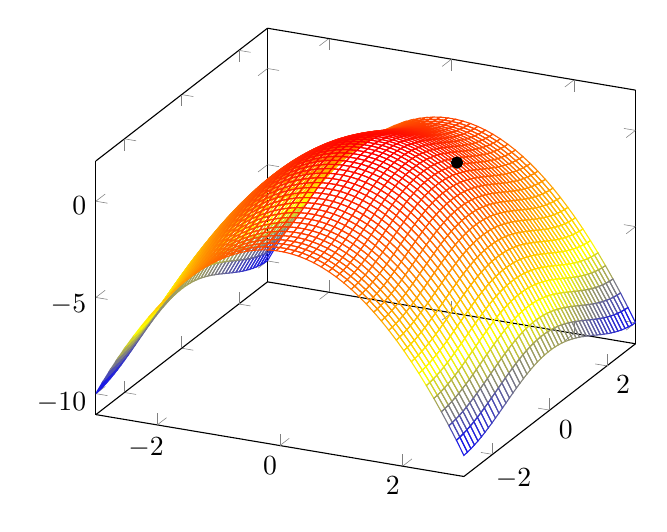
\begin{tikzpicture}
    \begin{axis}[]
        \addplot3[mesh, samples = 50, domain = -3:3]{cos(deg(y)) - x^2};
        \addplot3[black, mark=*] coordinates {(1, 1.047, -0.5)};
    \end{axis}
\end{tikzpicture}
    \caption{The surface $z = \cos{y} - x^2$}
    \label{fig:surface}
\end{figure}

We can see that $f(1, \pi/3) = -1/2$; therefore, the point $(1, \pi/3, -1/2)$ 
lies on the surface $z = \cos{y} - x^2$ (the black dot shown in figure \ref{
fig:surface}). If we fix $y$ such that $y = \pi/3$, we are looking at the 
intersection between the surface and the plane $y = \pi/3$ (see figure \ref{
fig:tangent}). 

\begin{figure}[htbp]
    \centering
    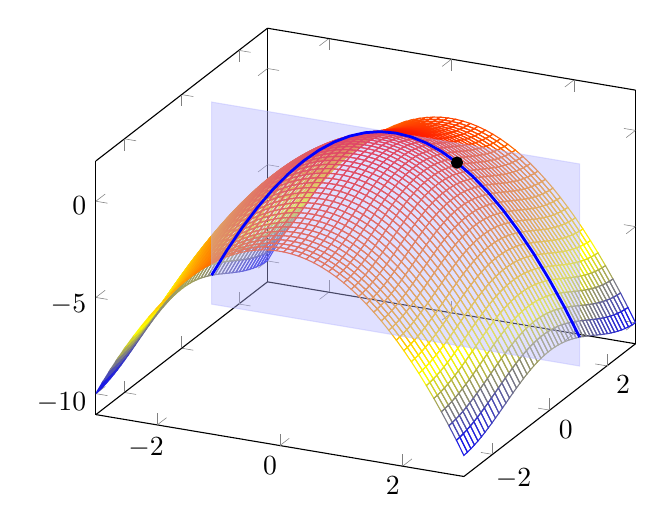
\begin{tikzpicture}
    \begin{axis}[]
        \addplot3[mesh, samples = 50, domain = -3:3]{cos(deg(y)) - x^2};
        \addplot3[black, mark=*] coordinates {(1, 1.047, -0.5)};
        \filldraw[blue!30, opacity = 0.4] (-3, 1.047, -10) -- (-3, 1.047, 0.5) 
        -- (3, 1.047, 0.5) -- (3, 1.047, -10) -- cycle;
        \addplot3+[draw=blue, line width = 1pt, domain = -3:3, samples y = 0, 
        mark=none] ({x}, 1.047, {0.5-x^2});
    \end{axis}
\end{tikzpicture}
    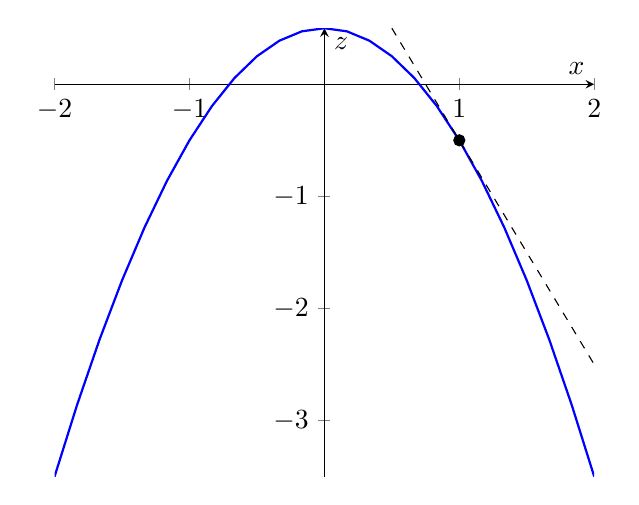
\begin{tikzpicture}
        \begin{axis}[axis lines = center, xlabel = $x$, ylabel = $z$]
            \addplot[blue, thick, domain = -2:2] {0.5-x^2};
            \addplot[black, thin, dashed, domain = 0.5:2] {-2*(x - 1) - 0.5};
            \addplot[black, mark=*] coordinates {(1, -0.5)};
        \end{axis}
    \end{tikzpicture}
    \caption{The intersection between the surface $z = \cos{y} - x^2$ and $y = 
    \pi/3$ is the parabola $z(x) = 1/2 - x^2$}
    \label{fig:tangent}
\end{figure}

We can describe this intersection as $g(x) = f(x, \pi/3)$, so the 
slope of a tangent line to this intersection is given by $g'(x) = f_x(x, 
\pi/3)$. This means, geometrically, $f_x(1, \pi/3)$ is the slope of the line 
that lies tangent to $z = f(x, y)$ at the point $(1, \pi/3, -1/2)$ and in the 
plane $y = \pi/3$ (see figure \ref{fig:tangent}). Alternatively, you could 
think of $f_x$ as the slope of the tangent line to the surface that is 
parallel to the $x$-axis. 

Similarly, we can fix $x = 1$ and look at the intersection between the surface 
$z = \cos{y} - x^2$ and the plane $x = 1$ (see figure \ref{fig:ytangent}. 
Just like before, we can describe this intersection as $h(y) = f(1, y)$, which 
means the slope of a line tangent to the intersection is given by $h'(y) = 
f_{y}(1, y)$. Therefore, as with $f_x$, $f_y(a, b)$ gives the slope of a line 
tangent to the point $\left(a, b, f(a, b) \right)$ and parallel to the $y$-axis. 

\begin{figure}[htbp]
    \centering
    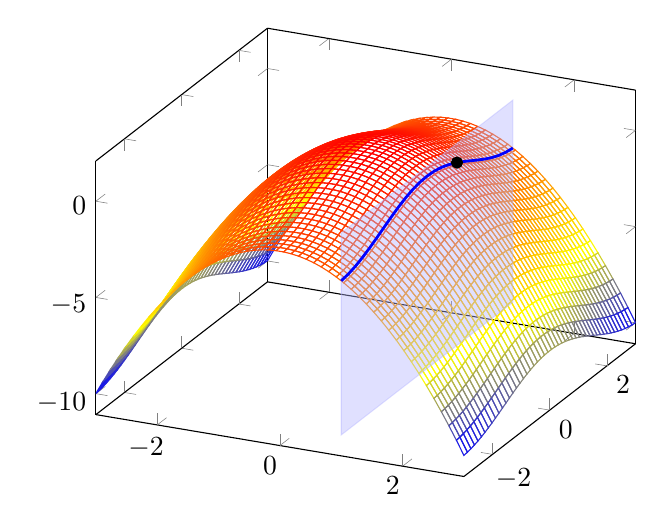
\begin{tikzpicture}
    \begin{axis}[]
        \addplot3[mesh, samples = 50, domain = -3:3]{cos(deg(y)) - x^2};
        \addplot3[black, mark=*] coordinates {(1, 1.047, -0.5)};
        \filldraw[blue!30, opacity = 0.4] (1, -3, -10) -- (1, -3, 0.5) 
        -- (1, 3, 0.5) -- (1, 3, -10) -- cycle;
        \addplot3+[draw=blue, line width = 1pt, domain = -3:3, samples y = 0, 
        mark=none] (1, {x}, {cos(deg(x))-1});
    \end{axis}
\end{tikzpicture}
    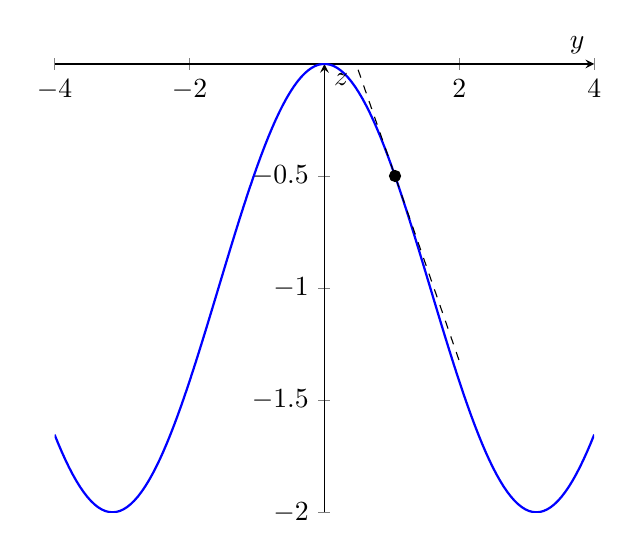
\begin{tikzpicture}
        \begin{axis}[axis lines = center, xlabel = $y$, ylabel = $z$]
            \addplot[blue, thick, domain = -4:4, samples = 150] 
            {cos(deg(x)) - 1};
            \addplot[black, thin, dashed, domain = 0.5:2] 
            {-0.866*(x - 1.047) - 0.5};
            \addplot[black, mark=*] coordinates {(1.047, -0.5)};
        \end{axis}
    \end{tikzpicture}
    \caption{The intersection between the surface $z = \cos{y} - x^2$ and 
    $x = 1$ is the trigonometric function $z = \cos{y} - 1$}
    \label{fig:ytangent}
\end{figure}

\textbf{Example}: The density of bacterial growth at a point $(x, y)$ on a 
flat agar plate is given by $D = 45/\left(2 + x^2 + y^2 \right)$. Find the 
rate of change of bacterial density at the point $(1, 3)$ (a) in the 
$x$-direction and (b) in the $y$-direction. Interpret the meaning of your 
results. 

\textbf{Solution}: The rate of change of a two-variable function in the 
$x$-direction is given by the partial derivative with respect to $x$:
$$D_x = \frac{\partial}{\partial x} \frac{45}{2 + x^2 + y^2} = \frac{-45 
\left( \partial/\partial x \right) \left(2 + x^2 + y^2 \right)}{\left(2 + 
x^2 + y^2 \right)^2}$$
$$= \frac{-90x}{\left( 2 + x^2 + y^2 \right)^2}$$

The rate of change in the $x$-direction at $(x, y) = (1, 3)$ is given by:
$$D_x(1, 3) = \frac{-90(1)}{\left( 2 + 1^2 + 3^2 \right)^2} = \frac{-90}{\left(
12 \right)^2} = \frac{-90}{144} = -\frac{5}{8}$$

This means that at $(1, 3)$, the density of bacteria is decreasing as you move 
away $x = 0$ along the line $y = 3$.

Similarly, the rate of change in the $y$-direction is given by the partial 
derivative with respect to $y$:
$$D_y = \frac{\partial}{\partial y} \frac{45}{2 + x^2 + y^2} = \frac{-45 \left(
\partial/\partial y \right) \left(2 + x^2 + y^2 \right)}{\left( 2 + x^2 + y^2 
\right)^2}$$
$$= \frac{-90y}{\left(2 + x^2 + y^2 \right)^2}$$

The rate of change in the $y$-direction at $(x, y) = (1, 3)$ is given by:
$$D_y(1, 3) = \frac{-90(3)}{\left(2 + 1^2 + 3^2 \right)^2} = \frac{-270}{144} 
= -\frac{15}{8}$$

This means that at $(1, 3)$ the density of bacteria is decreasing faster along 
the $y$-direction than along the $x$-direction. 

\begin{Exercise}[title = {Using partial derivatives to find tangent lines}, 
label = tangent]
Find equations for tangent lines to the surface at the given $xy$-coordinate. 
In which direction is the function changing the fastest?
\begin{enumerate}
\item $z = x^2e^{y/x}$, $(1, -1)$
\item $z = \cos{x} + y\sin{y}$, $(\pi, \pi/2)$
\item $z = x^2y - 3xy^2$, $(3, 2)$
\end{enumerate}
\vspace{75mm}
\end{Exercise}

\begin{Answer}[ref = tangent]
\begin{enumerate}
    \item $z(1, -1) = (1)^2e({-1/1} = 1/e$. Therefore, we are looking for 
    tangent lines through the point $(1, -1, 1/e)$. Finding a tangent line 
    parallel to the $x$-axis: $\frac{\partial z}{\partial x} = \frac{\partial}{
    \partial x} \left( x^2e^{y/x} \right) = x^2 \left( \frac{\partial}{\partial
    x}e^{y/x} \right) + e^{y/x} \left( \frac{\partial}{\partial x}x^2 \right) =
    x^2e^{y/x} \left( \frac{\partial}{\partial x} \frac{y}{x} \right) + 2x
    e^{y/x} = x^2 e^{y/x} \left( \frac{-y}{x^2} \right) + 2xe^{y/x} = \left( 
    2x - y \right)e^{y/x}$ and $z_x(1, -1) = \left( 2(1) - (-1) \right) 
    e^{-1/1} = \left(3 \right)e^{-1} = 3/e$. So, the slope of a line tangent to 
    the surface at $(1, -1, 1/e)$ parallel to the $x$-axis is $3/e$ and an 
    equation for that line is $z = 3/e \left(x - 1 \right) - 1/e$. 

    Finding a tangent line parallel to the $y$-axis: $\frac{\partial z}{
    \partial y} = \frac{\partial}{\partial y} \left( x^2e^{y/x} \right) = x
    e^{y/x}$ and $z_y(1, -1) = (1)e^{-1/1} = 1/e$. So, the slope of a line 
    tangent to the surface at $(1, -1, 1/e)$ parallel to the $y$-axis is $1/e$ 
    and an equation for that line is $z = 1/e \left(y + 1 \right) - 1/e$. 

    The function is changing faster in the $x$-direction. 

    \item $z(\pi, \pi/2) = \cos{(\pi)} + \frac{\pi}{2}\sin{(\pi/2)} = \frac{
    \pi}{2} - 1 $. Therefore, we are looking for tangent lines through the 
    point $(\pi, \pi/2, \pi/2 - 1)$. Finding a tangent line parallel to the 
    $x$-axis: $\frac{\partial z}{\partial x} = \frac{\partial}{\partial x} 
    \left( \cos{x} + y\sin{y} \right) = -\sin{x}$ and $z_x(\pi, \pi/2) = -\sin{
    \pi} = 0$. So, the slope of a line tangent to the surface at $(\pi, \pi/2, 
    \pi/2 - 1)$ parallel to the $x$-axis is $0$ and an equation for that line 
    is $z = \pi/2 - 1$.

    Finding a tangent line parallel to the $y$-axis: $\frac{\partial z}{
    \partial y} = \frac{\partial}{\partial y} \left( \cos{x} + y\sin{y} \right)
    = y \left( \frac{\partial}{\partial y}\sin{y} \right) + \sin{y} \left( 
    \frac{\partial}{\partial y} y \right) = y\cos{y} + \sin{y}$ and $z_y(\pi, 
    \pi/2) = \left( \frac{\pi}{2} \right) \cos{ \left( \frac{\pi}{2} \right) } 
    + \sin{ \left( \frac{\pi}{2} \right) } = 1$. So, the slope of a line tangent
    to the surface at $( \pi, \pi/2, \pi/2 - 1 )$ parallel to the $y$-axis is 
    $1$ and an equation for that line is $z = \left( y - \pi/2 \right) - \left(
    \pi/2 - 1 \right) = y - \pi + 1$. 

    The function is changing faster in the $y$-direction.

    \item $z(3, 2) = 3^2(2) - 3(3)(2^2) = 18 - 36 = -18$. Therefore, we are 
    looking for tangent lines through the point $(3, 2, -18)$. Finding a 
    tangent line parallel to the $x$-axis: $\frac{\partial z}{\partial x} = 
    \frac{\partial}{\partial x} \left( x^2y - 3xy^2 \right) = 2xy - 3y^2$ and 
    $z_x(3, 2) = 2(3)(2) - 3(2)^2 = 0$. So, the slope of a line tangent to the 
    surface at $(3, 2, -18)$ is $0$ and an equation for that line is $z = -18$

    Finding a tangent line parallel to the $y$-axis: $\frac{\partial z}{
    \partial y} = \frac{\partial}{\partial y} \left( x^2y - 3xy^2 \right) = 
    x^2 - 6xy$ and $z_y(3, 2) = 3^2 - 6(3)(2) = 9 - 36 = -27$. So, the slope of 
    a line tangent to the surface at $(3, 2, -18)$ is $-27$ and an equation for
    that line is $z = -27(y - 2) + -18 = -27y + 54 - 18 = 36 - 27y$.

    The function is changing faster in the $y$-direction. 
\end{enumerate}
\end{Answer}

\section{Gradient Vectors}
The gradient vector is used to find the direction of the maximum rate of change 
of a surface (for example, the steepest part of a mountain). In order to 
understand the gradient, we must first discuss directional derivatives. Recall 
that the partial derivatives, $f_x$ and $f_y$, can be used to define a plane 
tangent to the surface $z = f(x,y)$ (see figure \ref{fig:plane}). Directional 
derivatives allow us to find the slope of the tangent plane in directions 
other than the $x$- and $y$-directions. 

\begin{figure}[htbp]
    \centering
    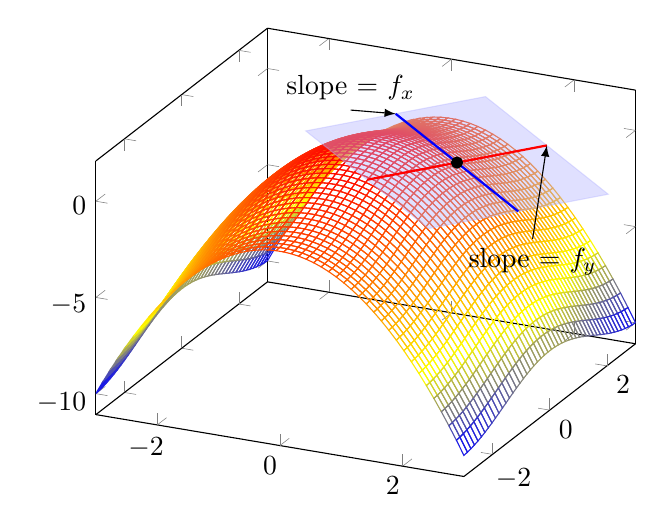
\begin{tikzpicture}
    \begin{axis}[]
        \addplot3[mesh, samples = 50, domain = -3:3]{cos(deg(y)) - x^2};
        \addplot3[black, mark=*] coordinates {(1, 1.047, -0.5)};
        \filldraw[blue!30, opacity = 0.4] (0, -2.094, 4.220) -- 
        (0, 4.189, -1.221) -- (2, 4.189, -5.221) -- (2, -2.094, 0.220) -- cycle;
        \draw[red, thick](1, -2.094, 2.220) -- (1, 4.189, -3.221);
        \draw[latex-] (0, 1.047, 1.5) -- (-0.5, 0.547, 2) node[above] {
        slope = $f_x$};
        \draw[blue, thick](0, 1.047, 1.5) -- (2, 1.047, -2.5);
        \draw[latex-](1, 4.189, -3.221) -- (2, 1.547, -4.5) node[below] {
        slope = $f_y$};
    \end{axis}
    \end{tikzpicture}
    \caption{The directional derivatives, $f_x$ and $f_y$ define a tangent 
    plane}
    \label{fig:plane}
\end{figure}

\subsection{Directional Derivatives}
The contour map in figure (FIXME make figure) shows the elevation, $H(x, y)$ 
for a mountain. You already know that you can use the partial derivatives, 
$H_x$ and $H_y$ to find the rate of change in elevation going east-west or 
north-south. But what about other directions? Suppose the hiking path you're 
on goes north-east. How can you predict the steepness (i.e. the rate of 
elevation change) along this path? The directional derivative allows us to 
find the rate of change in any direction. 

[explanation]

\begin{mdframed}[style = important, frametitle = {The Directional Derivative}]
Let $f$ be a differentiable function and \textbf{u} be a unit vector, 
$\textbf{u} = \left[ a, b \right]$. This means the directional derivative in the direction of 
\textbf{u} is:
$$D_u f(x, y) = f_x(x, y)a + f_y(x, y)b = \textbf{u}_x \left[ \frac{\partial}{
\partial x} f(x, y) \right] + \textbf{u}_y \left[ \frac{\partial}{\partial y} 
f(x, y) \right]$$
\end{mdframed}

Where $\textbf{u}_x$ and $\textbf{u}_y$ are the $x$- and $y$-components of 
\textbf{u}, respectively. 

\textbf{Example}: Find the directional derivative $D_u f(x, y)$ if $f(x, y) = 
y^3 - 3xy + 4x^2$ and \textbf{u} is the unit vector given by the angle $\theta 
= \pi/3$. What is the rate of change in the direction of \textbf{u} at $(1, 2)$?

\textbf{Solution}: We can describe \textbf{u} thusly:
$$\textbf{u} = \left[ \cos{ \frac{\pi}{3} }, \sin{ \frac{\pi}{3}} \right] = 
\left[ \frac{1}{2}, \frac{\sqrt{3}}{2} \right]$$

And therefore:
$$D_u f(x, y) = f_x(x, y) \left( \frac{1}{2} \right) + f_y(x, y) \left( \frac{
\sqrt{3}}{2} \right) $$
$$= \frac{\partial}{\partial x} \left( y^3 - 3xy + 4x^2 \right) \left( 
\frac{1}{2} \right) + \frac{\partial}{\partial y} \left( y^3 - 3xy + 4x^2 
\right) \left( \frac{\sqrt{3}}{2} \right)$$
$$= \frac{1}{2} \left( -3y + 8x \right) + \frac{\sqrt{3}}{2} \left( 3y^2 - 3x 
\right)$$
$$= \frac{-3}{2}y + 4x + \frac{3\sqrt{3}}{2}y^2 - \frac{3\sqrt{3}}{2}x = \frac{
3\sqrt{3}}{2}y^2 + \frac{8-3\sqrt{3}}{2}x - \frac{3}{2}y$$

And therefore $D_u f(1, 2)$ is:
$$= \frac{3\sqrt{3}}{2} \left( 2 \right)^2 + \frac{8 - 3\sqrt{3}}{2} \left( 1 
\right) - \frac{3}{2} \left( 2 \right) = 6\sqrt{3} + 4 - \frac{3\sqrt{3}}{2} - 
3$$
$$= 1 + \frac{9\sqrt{3}}{2}$$

\subsection{Unit Vectors in Two Dimensions}

What if the given vector is not a unit vector? We can scale the given vector 
to find a unit vector in the same direction:

\textbf{Example}: Find the directional derivative of $f(x, y) = 3x\sqrt{y}$ 
at $(1, 4)$ in the direction of $\textbf{v} = \left[2, 1 \right]$.

\textbf{Solution}: First, we need to find a unit vector in the same direction 
as \textbf{v}. There are several ways to do this. In two dimensions, a unit 
vector in the same direction as \textbf{v} can be found using trigonometry 
(see figure \ref{fig:vector} for an illustration). 

\begin{figure}[htbp]
    \centering
    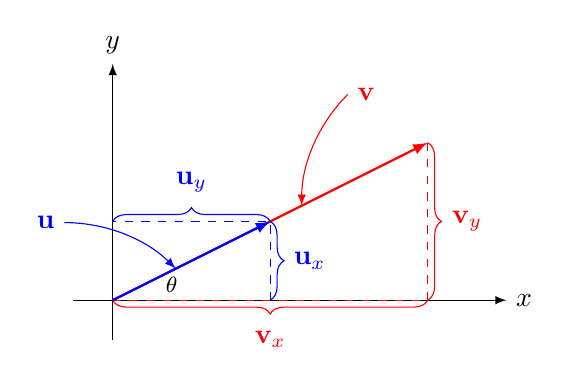
\begin{tikzpicture}
        \draw[black, -latex] (-0.5, 0) -- (5, 0) node[right] {$x$};
        \draw[black, -latex] (0, -0.5) -- (0, 3) node[above] {$y$};
        \draw[red, thick, -latex] (0, 0) -- (4, 2);
        \draw[red, thin, dashed] (0,0) -- (4, 0);
        \draw[red, thin, dashed] (4, 0) -- (4, 2);
        \draw[red, decorate, decoration = {brace, amplitude = 5pt, mirror}] 
        (0, 0) -- (4, 0) node[midway, yshift = -0.5cm] {$\textbf{v}_x$};
        \draw[red, decorate, decoration = {brace, amplitude = 5pt, mirror}] 
        (4, 0) -- (4, 2) node[midway, xshift = 0.5cm] {$\textbf{v}_y$};
        \draw[red, latex-] (2.4, 1.2) arc(180:135:2) node[right] {\textbf{v}};
        \draw[blue, thick, -latex] (0, 0) -- (2, 1);
        \draw[blue, latex-] (0.8, 0.4) arc(45:90:2) node[left] {\textbf{u}};
        \node[font = \footnotesize] at (0.75, 0.2) {$\theta$};
        \draw[blue, thin, dashed] (2, 0) -- (2, 1) -- (0, 1);
        \draw[blue, decorate, decoration = {brace, amplitude = 5pt, mirror}] 
        (2, 0) -- (2, 1) node[midway, xshift = 0.5cm] {$\textbf{u}_x$};
        \draw[blue, decorate, decoration = {brace, amplitude = 5pt}] 
        (0, 1) -- (2, 1) node[midway, yshift = 0.5cm] {$\textbf{u}_y$};
    \end{tikzpicture}
    \caption{\textbf{u} is a unit vector in the same direction as \textbf{v}}
    \label{fig:vector}
\end{figure}

We know that $\theta = \arctan{ \left( \textbf{v}_y / \textbf{v}_x \right)}$. 
Therefore, the $x$-component of the unit vector, \textbf{u}, is given by:
$$\textbf{u}_x = |\textbf{u}| \cos{ \theta} = \cos{ \left( \arctan{ \frac{
\textbf{v}_y}{\textbf{v}_x}} \right)}$$

Similarly, we know that:
$$\textbf{u}_y = |\textbf{u}| \sin{ \theta} = \sin{ \left( \arctan{ \frac{
\textbf{v}_y}{\textbf{v}_x}} \right)}$$

(Recall that since \textbf{u} is a unit vector, $|\textbf{u}| = 1$). 

Let's use this method to find a unit vector, \textbf{u}, in the same direction 
as $\textbf{v} = \left[ 2, 1 \right]$:
$$\textbf{u}_x = \cos{ \left( \arctan{ \frac{1}{2} } \right) } \approx \cos{ 
\left( 0.464 \right) } = \frac{2}{\sqrt{5}}$$
$$\textbf{u}_y = \sin{ \left( \arctan{ \frac{1}{2} } \right) } \approx \sin{ 
\left( 0.464 \right)} = \frac{1}{\sqrt{5}}$$

Therefore, a unit vector in the same direction as \textbf{v} is $\textbf{u} = 
\left[ 2/\sqrt{5}, 1/\sqrt{5} \right]$. 

And we can find the directional derivative:
$$D_u(x, y) = \textbf{u}_x \left[ \frac{\partial}{\partial x} f(x, y) \right] 
+ \textbf{u}_y \left[ \frac{\partial}{\partial y} f(x, y) \right]$$
$$D_u(x, y) = \left( \frac{2}{\sqrt{5}} \right) \left[ \frac{\partial}{
\partial x} \left( 3x\sqrt{y} \right) \right] + \left( \frac{1}{\sqrt{5}} 
\right) \left[ \frac{\partial}{\partial y} \left( 3x\sqrt{y} \right) \right]$$
$$D_u(x, y) = \left( \frac{2}{\sqrt{5}} \right) \left( 3\sqrt{y} \right) + 
\left( \frac{1}{\sqrt{5}} \right) \left( \frac{3x}{2\sqrt{y}} \right)$$
$$D_u(x, y) = \frac{12y + 3x}{2\sqrt{5y}}$$

To find the magnitude of the directional derivative at $(1, 4)$, we 
substitute for $x$ and $y$:
$$D_u(1, 4) = \frac{12(4) + 3(1)}{2\sqrt{5(4)}} = \frac{51}{4\sqrt{5}} 
\approx 5.702$$

\subsection{Unit Vectors in Higher Dimensions}
The trigonometric explanation for finding unit vectors is more difficult to visualize in higher dimensions. However, there is another method that works well in 2, 3, and higher dimensions. Recall that the magnitude of a vector, $\textbf{v} = \left[ \textbf{v}_x, \textbf{v}_y \right]$ is given by $| \textbf{v} | = \sqrt{\left( \textbf{v}_x \right)^2 + \left( \textbf{v}_y \right)^2}$. For a vector with $n$ dimensions, $\textbf{v} = \left[ \textbf{v}_1, \textbf{v}_2, \cdots , \textbf{v}_n \right]$, the magnitude is given by $| \textbf{v} | = \sqrt{ \left( \textbf{v}_1 \right)^2 + \left( \textbf{v}_2 \right)^2 + \cdots + \left( \textbf{v}_n \right)^2}$. 

To find a unit vector, \textbf{u}, in the same direction as \textbf{v}, we can scale \textbf{v} up or down so that its magnitude is 1. We can do this by dividing by \textbf{v}'s magnitude. Consider the two-dimensional vector used in the last example, $\textbf{v} = \left[ 2, 1 \right]$. Its magnitude is:
$$| \textbf{v} | = \sqrt{\left( 2 \right)^2 + \left( 1 \right)^2} = \sqrt{5}$$

Let's check if $\textbf{v} / | \textbf{v} |$ is a unit vector:
$$ \frac{\textbf{v}}{|\textbf{v}|} = \left( \frac{1}{\sqrt{5}} \right) \left[ 2, 1 \right] = \left[ \frac{2}{\sqrt{5}}, \frac{1}{\sqrt{5}} \right]$$

And the magnitude of this scaled vector is:
$$ \left| \frac{\textbf{v}}{| \textbf{v} |} \right| = \sqrt{\left( \frac{2}{\sqrt{5}} \right)^2 + \left( \frac{1}{\sqrt{5}} \right)^2} = \sqrt{\frac{4}{5} + \frac{1}{5}} = \sqrt{1} = 1$$

Notice our unit vector is the same as we found using the trigonometric method above. 

Another way to think of the question is: What factor, $k$, can we multiply \textbf{v} by to yield a vector with a magnitude of 1? Let's see this method for the 3-dimensional vector $\textbf{v} = \left[ 3, 2, 1 \right]$. We are looking for a $k$ such that:
$$|k\textbf{v}| = 1$$
$$|k \textbf{v}| = \left| \left[ 3k, 2k, 1k \right] \right| = \sqrt{\left( 3k \right)^2 + \left( 2k \right)^2 + \left( 1k \right)^2}$$
$$= \sqrt{9k^2 + 4k^2 + k^2} = k\sqrt{14} = 1$$

Which implies that $k = 1/\sqrt{14}$, which is $1/|\textbf{v}|$. Therefore, a unit vector in the same direction as $\textbf{v} = \left[ 3, 2, 1 \right]$ is:
$$\textbf{u} = \frac{1}{\sqrt{14}} \left[ 3, 2, 1 \right] = \left[ \frac{3}{\sqrt{14}}, \frac{2}{\sqrt{14}}, \frac{1}{\sqrt{14}} \right]$$


\begin{Exercise}[title = {Finding Directional Derivatives}, label = direction]
Find the directional derivative of the function at the given point in the 
direction of the given vector. 
\begin{enumerate}
    \item $f(x, y) = e^{3x} \sin{2y}$, $(0, \pi/6)$, $\textbf{v} = \left[ -3, 
    4 \right]$
    \item $f(x, y) = x^2y + xy^3$, $(2, 4)$, $\textbf{v} = 2 \textbf{i} - 
    \textbf{j}$
    \item $f(x, y, z) = \ln{ \left( x^2 + 3y - z \right)}$, $(2, 2, 1)$, 
    $\textbf{v} = \left[ 1, 1, 1 \right]$
\end{enumerate}
\vspace{100mm}
\end{Exercise}

\begin{Answer}[ref = direction]
\begin{enumerate}
    \item First, we define \textbf{u} such that $|\textbf{u}| = 1$ and 
    \textbf{u} is in the same direction as \textbf{v}:
    $$\textbf{u} = k \textbf{v} = \left[ -3k, -4k \right]$$
    $$\sqrt{ \left( -3k \right)^2 + \left( 4k \right)^2} = 1$$
    $$\sqrt{9k^2 + 16k^2} = \sqrt{25k^2} = 5k = 1$$
    $$k = \frac{1}{5}$$

    Therefore, we define $\textbf{u} = \left[ -3/5, 4/5 \right]$ and the 
    directional derivative is given by:
    $$D_u(x, y) = \left( \frac{-3}{5} \right) \frac{\partial}{\partial x} f(x, 
    y) + \left( \frac{4}{5} \right) \frac{\partial}{\partial y} f(x, y)$$
    $$= \left( \frac{-3}{5} \right) \frac{\partial}{\partial x} \left[ e^{3x} 
    \sin{2y} \right] + \left( \frac{4}{5} \right) \frac{\partial}{\partial y} 
    \left[ e^{3x} \sin{2y} \right]$$
    $$= \left( \frac{-3}{5} \right) \left( 3e^{3x} \sin{2y} \right) + \left( 
    \frac{4}{5} \right) \left( 2e^{3x} \cos{2y} \right)$$

    And substituting for $(x, y) = (0, \pi/6)$:
    $$D_u(0, \pi/6) = \left( \frac{-3}{5} \right) \cdot \left[ 3e^{3 \cdot 0} 
    \sin{ \left( \frac{\pi}{3} \right)} \right] + \left( \frac{4}{5} \right) 
    \cdot \left[ 2e^{3 \cdot 0} \cos{ \left( \frac{\pi}{3} \right)} \right]$$
    $$D_u(0, \pi/6) = \left( \frac{-3}{5} \right) \cdot \left[ 3 \cdot \frac{
    \sqrt{3}}{2} \right] + \left( \frac{4}{5} \right) \cdot \left[ 2 \cdot 
    \frac{1}{2} \right]$$
    $$d_u(0, \pi/6) = \left( \frac{-3}{5} \right) \cdot \left( \frac{3
    \sqrt{3}}{2} \right) + \left( \frac{4}{5} \right) \cdot \left( 1 \right)$$
    $$D_u(0, \pi/6) = \frac{-9\sqrt{3}}{10} + \frac{8}{10} = \frac{8-9\sqrt{3}
    }{10} \approx -0.759$$

    \item We can express \textbf{v} as $\textbf{v} = \left[ 2, -1 \right]$. 
    And we define \textbf{u} such that $| \textbf{u} | = 1$ and \textbf{u} is 
    in the same direction as \textbf{v}:
    $$\textbf{u} = k\textbf{v} = \left[ 2k, -k \right]$$
    $$\sqrt{\left( 2k \right)^2 + \left( -k \right)^2} = 1$$
    $$\sqrt{4k^2 + k^2} = \sqrt{5}k = 1$$
    $$k = \frac{1}{\sqrt{5}} = \frac{\sqrt{5}}{5}$$

    Therefore, we define $\textbf{u} = \left[ 2\sqrt{5}/5, -\sqrt{5}/5 \right]$
    and the directional derivative is given by:
    $$D_u(x, y) = \left( \frac{2\sqrt{5}}{5} \right) \frac{\partial}{\partial 
    x}f(x, y) + \left( \frac{-\sqrt{5}}{5} \right) \frac{\partial}{\partial y}
    f(x, y)$$
    $$= \left( \frac{2\sqrt{5}}{5} \right) \frac{\partial}{\partial x} \left[ 
    x^2y + xy^3 \right] + \left( \frac{-\sqrt{5}}{5} \right) \frac{\partial}{
    \partial y} \left[ x^2y + xy^3 \right]$$
    $$= \left( \frac{2\sqrt{5}}{5} \right) \left[ 2xy + y^3 \right] + \left( 
    \frac{-\sqrt{5}}{5} \right) \left[ x^2 + 3xy^2 \right]$$

    And substituting $(x, y) = (2, 4)$:
    $$D_u(2, 4) = \left( \frac{2\sqrt{5}}{5} \right) \left[ 2(2)(4) + 4^3 
    \right] + \left( \frac{-\sqrt{5}}{5} \right) \left[ 2^2 + 3(2)(4^2) 
    \right]$$
    $$D_u(2, 4) = \left( \frac{2\sqrt{5}}{5} \right) \left[ 80 \right] + \left(
    \frac{-\sqrt{5}}{5} \right) \left[ 100 \right]$$
    $$D_u(2, 4) = 32\sqrt{5} - 20\sqrt{5} = 12\sqrt{5} \approx 26.833$$

    \item We define \textbf{u} such that $| \textbf{u} | = 1$ and \textbf{u} 
    is in the same direction as \textbf{v}:
    $$\textbf{u} = k\textbf{v} = \left[k, k, k \right]$$
    $$\sqrt{k^2 + k^2 + k^2} = 1$$
    $$\sqrt{3}k = 1$$
    $$k = \frac{1}{\sqrt{3}} = \frac{\sqrt{3}}{3}$$

    Therefore, we let $\textbf{u} = \left[ \sqrt{3}/3, \sqrt{3}/3, \sqrt{3}/3 
    \right]$ and the directional derivative is given by:
    $$D_u(x, y, z) = \left( \frac{\sqrt{3}}{3} \right) \frac{\partial}{
    \partial x} f(x, y, z) + \left( \frac{\sqrt{3}}{3} \right) \frac{
    \partial}{\partial y}f(x, y, z) + \left( \frac{\sqrt{3}}{3} \right) 
    \frac{\partial}{\partial z} f(x, y, z)$$
    $$= \left( \frac{\sqrt{3}}{3} \right) \left[ \frac{\partial}{\partial x} 
    \ln{ \left( x^2 + 3y - z \right)} + \frac{\partial}{\partial y} \ln{ 
    \left( x^2 + 3y - z \right)} + \frac{\partial}{\partial z} \ln{ \left( 
    x^2 + 3y - z \right)} \right]$$
    $$= \left( \frac{\sqrt{3}}{3} \right) \left[ \frac{2x}{x^2 + 3y - z} + 
    \frac{3}{x^2 + 3y - z} + \frac{-1}{x^2 + 3y - z} \right]$$
    $$= \left( \frac{\sqrt{3}}{3} \right) \left[ \frac{2x + 2}{x^2 + 3y - z} 
    \right] = \frac{\sqrt{3} \left( 2x + 2 \right)}{3 \left( x^2 + 3y - z 
    \right)}$$

    And substituting $(x, y, z) = (2, 2, 1)$:
    $$D_u(2, 2, 1) = \frac{\sqrt{3} \left( 2(2) + 2 \right)}{3 \left( 2^2 + 
    3(2) - 1 \right)} = \frac{\sqrt{3} \left( 6 \right)}{3 \left( 9 \right)} 
    = \frac{2\sqrt{3}}{9} \approx 0.385$$
\end{enumerate}
\end{Answer}

\subsection{Maximizing the Gradient}
The directional derivative can be written as the dot product of two vectors:
$$D_u f(x, y) = af_x(x, y) + bf_y(x, y) = \left[ f_x(x, y), f_y(x, y) \right] 
\cdot \textbf{u}$$

The first vector, $\left[ f_x(x, y), f_y(x, y) \right]$, is called \textit{the 
gradient of f}\index{gradient}, and is noted as $\nabla f$. 

\begin{mdframed}[style = important, frametitle = {The Gradient}]
For a two-variable function, $f(x, y)$, the gradient of $f$ is the vector:
$$\nabla f = \left[ f_x(x, y), f_y(x, y) \right] = \frac{\partial f}{\partial 
x} \textbf{i} + \frac{\partial f}{\partial y} \textbf{j}$$

Where \textbf{i} and \textbf{j} are the unit vectors in the $x$- and 
$y$-directions, respectively.
\end{mdframed}

Think back to the elevation example we opened the chapter with. What if we 
wanted to complete our ascent as quickly as possible? We would want to 
know the direction in which the elevation is changing the fastest. This occurs 
when the direction we are going is the same direction as the gradient vector, 
$\nabla f$. 

Recall that the dot product is defined as:
$$\textbf{u} \cdot \textbf{v} = \left| \textbf{u} \right| \left| \textbf{v} 
\right| \cos{ \theta}$$

Where $\theta$ is the angle between the vectors \textbf{u} and \textbf{v}. 
Applying this to the directional derivative, we see that:
$$D_u f = \nabla f \cdot \textbf{u} = \left| \nabla f \right| \left| 
\textbf{u} \right| \cos{\theta} = \left| \nabla f \right| \cos{\theta}$$

Which is at its maximum when $\nabla f$ and \textbf{u} point in the same 
direction (because $\cos{\left( 0 \right)} = 1$). Therefore, the gradient 
vector points in the direction of maximum change and the magnitude of that 
vector is the rate of maximum change. 

\textbf{Example}: Find the maximum rate of change of $f(x, y) = 4y\sqrt{x}$ at 
$(4, 1)$. In what direction does the maximum change occur?

\textbf{Solution}: We begin by finding $\nabla f$:
$$\nabla f = \left[ \frac{\partial}{\partial x} \left( 4y\sqrt{x} \right), 
\frac{\partial}{\partial y} \left( 4y\sqrt{x} \right) \right]$$
$$\nabla f = \left[ \frac{2y}{\sqrt{x}}, 4\sqrt{x} \right]$$

And thus, 
$$\nabla f(4, 1) = \left[ \frac{2(1)}{\sqrt{4}}, 4\sqrt{4} \right] = \left[ 1, 
8 \right]$$

Therefore, the maximum value of $\nabla f$ at $(4, 1)$ is:
$$\left| \nabla f \right| = \sqrt{1^2 + 8^2} = \sqrt{65}$$

in the direction of the vector $\left[ 1, 8 \right]$. 

\begin{Exercise}[title = {Using the Gradient to find Maximum Change}, 
label = maximum]
Suppose you are climbing a mountain whose elevation is described by $z = 3000 
- 0.01x^2 - 0.02y^2$. Take the positive $x$-direction to be east and the 
positive $y$-direction to be north. 
\begin{enumerate}
    \item If you are at $(x, y) = (50, 50)$, what is your elevation?
    \item If you walk south, will you ascend or descend?
    \item If you walk northwest, will you ascend or descend? Will the rate of 
    elevation change be greater or less than if you walked south?
    \item In what direction should you walk for the steepest ascent? What will 
    your ascension rate be?
\end{enumerate}
\vspace{50mm}
\end{Exercise}

\begin{Answer}[ref = maximum]
\begin{enumerate}
    \item $z = f(50, 50) = 3000 - 0.01(50)^2 - 0.02(50)^2 = 2925$
    \item A south-pointing unit vector is $\textbf{u} = \left[ 0, -1 \right]$. 
    To find the rate of change, we find the directional derivative in the 
    direction of \textbf{u} at $(50, 50)$:
    $$D_u f(x, y) = \left( -1 \right) \left[ \frac{\partial}{\partial y} 
    \left( 3000 - 0.01x^2 - 0.02y^2 \right) \right]$$
    $$D_u f(x, y) = \left( -1 \right) \left( -0.04 y \right) = 0.04y$$

    And at $(50, 50)$, $D_u f(50, 50) = 0.04(50) = 2 > 0$. Therefore, if you 
    walk south, you will ascend.
    \item A northwest-pointing unit vector is $\textbf{u} = \left[ -\sqrt{2}
    /2, \sqrt{2}/2 \right]$. To find the rate of change, we find the 
    directional derivative at $(50, 50)$ in the direction of \textbf{u}:
    $$D_u f(x, y) = \left( \frac{-\sqrt{2}}{2} \right) \left[ \frac{\partial}{
    \partial x} f(x, y) \right] + \left( \frac{\sqrt{2}}{2} \right) \left[ 
    \frac{\partial}{\partial y} f(x, y) \right]$$
    $$D_u f(x, y) = \left( \frac{-\sqrt{2}}{2} \right) \left[ -0.02x \right] 
    + \left( \frac{\sqrt{2}}{2} \right) \left[ -0.04 y \right]$$
    $$D_u f(x, y) = 0.01\sqrt{2}x - 0.02\sqrt{2}y$$
    $$D_u f(50, 50) = 0.01 \sqrt{2} \left( 50 \right) - 0.02 \sqrt{2} \left( 
    50 \right) = \frac{-\sqrt{2}}{2} \approx -0.707$$

    The rate of elevation change walking northwest is approximately $-0.707$, 
    so you will descend and your rate of elevation change would be less than 
    if you walked south. 

    \item To find the direction of maximum elevation gain, we find the 
    direction the gradient vector points in:
    $$\nabla f = \left[ \frac{\partial f}{\partial x}, \frac{\partial f}{
    \partial y} \right]$$
    $$\nabla f = \left[ -0.02x, -0.04y \right]$$

    And at $(50, 50)$, 
    $$\nabla f(50, 50) = \left[ -0.02(50), -0.04(50) \right] = \left[ -1, -2 
    \right]$$

    Therefore, the rate of greatest elevation change is in a south-by-southwest 
    direction indicated by the vector $\left[ -1, -2 \right]$ and the rate of 
    elevation change is $\left| \nabla f(50, 50) \right| = \sqrt{(-1)^2 + (-2)^
    2} = \sqrt{5}$. Notice this is greater than the other two rates of change 
    we have found. 
\end{enumerate}
\end{Answer}

\section{Applications of Partial Derivatives and Gradients}

\subsection{Laplace's Equation}